\documentclass{article}

%Page format
\usepackage[table]{xcolor}
\usepackage{pdfpages}
\usepackage{fancyhdr}
\usepackage[margin=1in]{geometry}
\usepackage{tabularx}
%Math packages and custom commands
\usepackage{algpseudocode}
\usepackage{amsthm}
\usepackage{framed}
\usepackage[margin=1in]{geometry}
\usepackage{hyperref}
\usepackage{tikz}
\usepackage[utf8]{inputenc}
\definecolor{Gray}{gray}{0.9}
\usepackage{wrapfig}
\usepackage[margin=1in]{geometry}
\usepackage{mathtools,amsthm}
\usepackage{enumitem,amssymb}
\newtheoremstyle{case}{}{}{}{}{}{:}{ }{}
\theoremstyle{case}
\newtheorem{case}{Case}
\DeclareMathOperator{\R}{\mathbb{R}}
\DeclareMathOperator{\E}{\mathbb{E}}
\DeclareMathOperator{\Var}{\text{Var}}
\DeclareMathOperator{\Cov}{\text{Cov}}
\newcommand{\bvec}[1]{\mathbf{#1}}
\renewcommand{\P}{\mathbb{P}}
\newcommand{\norm}[2][2]{\| #2\|_{#1}}

\definecolor{shadecolor}{gray}{0.9}

\theoremstyle{definition}
\newtheorem*{answer}{Answer}
\newcommand{\note}[1]{\medskip \noindent{\textbf{NOTE:} #1}}
\newcommand{\hint}[1]{\medskip \noindent{\textit{HINT:} #1}}
\newcommand{\recall}[1]{\medskip{[\textbf{RECALL:} #1]}}
\newcommand{\motivation}[1]{\medskip \noindent{\textbf{MOTIVATION:} #1}}
\newcommand{\expect}[1]{\medskip \noindent{\fbox{\parbox{0.95 \textwidth}{\medskip \textbf{What we expect:} #1}}}}
\newcommand{\mysolution}[1]{\noindent{\begin{shaded}\textbf{Your Solution:}\ #1 \end{shaded}}}
\newlist{todolist}{itemize}{2}
\setlist[todolist]{label=$\square$}
\usepackage{pifont}
% use below to modify the size of equations
% usage is as follows: {fontsize}{math text size}{subscript size}{subsubscript size}
% if you wish to change the math font size, modify {math text size}{subscript size}{subsubscript size} for your chosen global font size {fontsize} which is declared at the beginning of the document
%\DeclareMathSizes{10}{13}{13}{13}
%\DeclareMathSizes{14}{17}{17}{17}
%\DeclareMathSizes{12}{15}{15}{15}
\newcommand{\cmark}{\ding{51}}%
\newcommand{\xmark}{\ding{55}}%
\newcommand{\done}{\rlap{$\square$}{\raisebox{2pt}{\large\hspace{1pt}\cmark}}%
\hspace{-2.5pt}}
\newcommand{\wontfix}{\rlap{$\square$}{\large\hspace{1pt}\xmark}}
\graphicspath{ {./images/} }

\title{\textbf{CS221 Spring 2024: Artificial Intelligence:\\ Principles and Techniques} \\Homework 6: Scheduling}
\date{}

\chead{Scheduling}
\rhead{\today}
\lfoot{}
\cfoot{CS221: Artificial Intelligence: Principles and Techniques --- Spring 2024}
\rfoot{\thepage}
\renewcommand{\headrulewidth}{0.4pt}
\renewcommand{\footrulewidth}{0.4pt}
\pagestyle{fancy}
\setlength{\parindent}{0pt}

\begin{document}

\maketitle

\begin{center}
\begin{tabular}{rl}
SUNet ID: & [your SUNet ID] \\
Name: & [your first and last name] \\
Collaborators: & [list all the people you worked with]
\end{tabular}
\end{center}
\newcolumntype{g}{>{\columncolor{Gray}}c}
\textit{By turning in this assignment, I agree by the Stanford honor code and declare
that all of this is my own work.} \\
% uncomment one of the below lines to make the text larger
\fontsize{12pt}{16pt}\selectfont
% \fontsize{14pt}{18pt}\selectfont

\section*{Problem 0: CSP basics}

\begin{enumerate}[label=\alph*.]
\item
{[4 points]} Let's create a CSP. Suppose you have $n$ light bulbs, where each light bulb $i=1,\dots,n$ is initially off. You also have $m$ buttons which control the lights. For each button $j=1,\dots,m$, we know the subset $T_j \subseteq \{ 1, \dots, n \}$ of light bulbs that it controls. When button $j$ is pressed, it toggles the state of each light bulb in $T_j$ (for example, if $3 \in T_j$ and light bulb 3 is off, then after the button is pressed, light bulb 3 will be on, and vice versa). If multiple---say $Z$ buttons---controlling the same light bulb are pressed, then that light bulb will be turned on if $Z$ is odd, or it will be turned off if $Z$ is even.
	
Your goal is to turn on all the light bulbs by pressing a subset of the buttons. Construct a CSP to solve this problem. Your CSP should have $m$ variables and $n$ constraints. \textit{For this problem only}, you can use $m$-ary constraints: constraints that can be functions of up to $m$ variables. Describe your CSP precisely and concisely. You need to specify the variables with their domain, and the constraints with their scope and expression. Make sure to include $T_j$ in your answer. 
	
Hint: If stuck, take a look at parts (b) and (c) of this problem to see how you could define the constraints using a boolean operator.
	
\expect{

What are the $m$ variables and their domains. What do they represent?

What are the $n$ constraints and what do they mean?
}
% Problem 0a
\mysolution

\item
{[6 points]} Now, let's consider a simple CSP with 3 variables and 2 binary factors:
	\begin{center}
	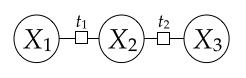
\includegraphics{scheduling-0-a}
	\end{center}
	where $X_1, X_2, X_3 \in \{ 0, 1\}$ and $t_1, t_2$ are $\mathsf{XOR}$ functions (that is $t_1(X) = x_1 \oplus x_2$ and $t_2(X) = x_2 \oplus x_3$). 
	\begin{enumerate}[label=\roman*.]
	\item
		What are the consistent assignments for this CSP?
	\item
Let's use backtracking search to solve the CSP. The \texttt{Backtrack()} algorithm as defined in the lectures is a recursive algorithm, where new instances of \texttt{Backtrack()} are called within parent instances of \texttt{Backtrack()}.
	
In this problem, we will ask you to produce the call stack for a specific call to \texttt{Backtrack()}. A call stack is just a diagram tracing out every recursive call. For our purposes, for each call to \texttt{Backtrack()} you should specify which variable is being assigned, the current domains, and which parent call to \texttt{Backtrack()} it's called within. For example, if the order in which we assign variables is $X_1, X_2, X_3$, the call stack would be as follows:
	\begin{align*}
	&\{[01], [01], [01]\} \quad &\overset{X_1 = 0}{\longrightarrow} \quad &\{\textbf{0}, [01], [01]\} \quad &\overset{X_2 = 1}{\longrightarrow} \quad &\{\textbf{0}, \textbf{1}, [01]\} \quad &\overset{X_3 = 0}{\longrightarrow} \quad &\{ \textbf{0}, \textbf{1}, \textbf{0}\} \\
	 \cline{1-8} \\
	& &\overset{X_1 = 1}{\longrightarrow} \quad &\{\textbf{1}, [01], [01]\} \quad &\overset{X_2 = 0}{\longrightarrow} \quad &\{\textbf{1}, \textbf{0}, [01]\} \quad &\overset{X_3 = 1}{\longrightarrow} \quad &\{ \textbf{1}, \textbf{0}, \textbf{1}\}
	\end{align*}
	The notation $\{\textbf{1}, [01], [01]\}$ means that $X_1$ has been assigned value 1, while $X_2$ and $X_3$ are currently unassigned and each have domain $\{0,1\}$. Note that we omit the comma in the domain for easier reading. We also avoid the weight variable for simplicity; the only possible weights for this problem are 0 and 1. In this case, backtrack is called 7 times. Notice that \texttt{Backtrack()} is not called when there's an inconsistent partial assignment ($\delta=0$); for example, we don't call \texttt{Backtrack()} on $X_2=1$ when $X_1$ is already set to 1. 
	
	Using this call stack, we can produce the list of calls in the order they are explored. For this example where we assign variables in order $X_1, X_2, X_3$, the list would be
	\begin{align*}
	\{[01],[01],[01]\},\{0,[01],[01]\},\{0,1,[01]\},\{0,1,0\},\{1,[01],[01]\},\{1,0,[01]\},\{1,0,1\}.
	\end{align*}
	
	Suppose we assign variables in the order $X_3, X_1, X_2$. Write the list of calls in the order they are explored and draw out the call-stack. How many calls do we make to \texttt{Backtrack()}? Why can this number change depending on the ordering? In keeping with the given example, you should run \texttt{Backtrack()} to find all consistent assignments.
	\item
	We often add heuristics like AC-3 to speed up the backtracking search. How many calls to \texttt{Backtrack()} from your call stack in the previous question would we skip if we use AC-3? Briefly explain why we skip (or don't skip) calls in this search with AC-3. 
	\end{enumerate}
	\expect{
 
	(i.) A list of all the consistent assignments (1 sentence).

	(ii.) A list of calls in order of exploration.

	(ii.) A drawing of the call stack.

	(ii.) The number of times Backtrack() is called, an explanation for why this number can change based on the order in which you assign variables (1-4 sentences).

	(iii.) The number of calls to Backtrack() that get skipped along with an explanation for why we skip these calls with AC-3 (1-2 sentences).

	}
	% Problem 0b
	\mysolution

\item
{[2 points]} Now let's consider a general case: given a factor graph with $n$ variables $X_1,\dots,X_n$ and $n-1$ binary factors $t_1,\dots,t_{n-1}$ where $X_i \in \{0,1\}$ and $t_i(X)=x_i\oplus x_{i+1}$. Note that the CSP has a chain structure. Implement \texttt{create\_chain\_csp()} by creating a generic chain CSP with XOR as factors.

\textbf{Note:} We've provided you with a CSP implementation in \texttt{util.py} which supports unary and binary factors. For now, you don't need to understand the implementation, but please read the comments and get yourself familiar with the CSP interface. For this problem, you'll need to use \texttt{CSP.add\_variable()} and \texttt{CSP.add\_binary\_factor()}. 
\end{enumerate}

\newpage
\section*{Problem 1: CSP solving}
We'll now pivot towards creating more complicated CSPs, and solving them faster using heuristics. Notice we are already able to solve the CSPs because in \texttt{submission.py}, a basic backtracking search is already implemented. For this problem, we will work with \textit{unweighted} CSPs that can only have True/False factors; a factor outputs 1 if a constraint is satisfied and 0 otherwise. The backtracking search operates over partial assignments, and specifies whether or not the current assignment satisfies all relevant constraints. When we assign a value to a new variable $X_i$, we check that all constraints that depend only on $X_i$ and the previously assigned variables are satisfied. The function \texttt{satisfies\_constraints()} returns whether or not these new factors are satisfied based on the \texttt{unaryFactors} and \texttt{binaryFactors}. When \texttt{satisfies\_constraints()} returns False, any full assignment that extends the new partial assignment cannot satisfy all of the constraints, so \textit{there is no need to search further with that new partial assignment}.

Take a look at \texttt{BacktrackingSearch.reset\_results()} to see the other fields which are set as a result of solving the weighted CSP. You should read \texttt{submission.BacktrackingSearch} carefully to make sure that you understand how the backtracking search is working on the CSP. 

\begin{enumerate}[label=\alph*.]
    \item
    {[5 points]} Let's create an unweighted CSP to solve the n-queens problem: Given an $n\times n$ board, we'd like to place $n$ queens on this board such that no two queens are on the same row, column, or diagonal. Implement \texttt{create\_nqueens\_csp()} by \textbf{adding $n$ variables} and some number of binary factors. Note that the solver collects some basic statistics on the performance of the algorithm. You should take advantage of these statistics for debugging and analysis. You should get 92 (optimal) assignments for $n=8$ with exactly 2057 operations (number of calls to \texttt{backtrack()}).

Hint: If you get a larger number of operations or your code times out on the test cases, make sure your CSP is minimal. Try to define the variables such that the size of domain is $O(n)$.

Note: Please implement the domain of variables as 'list' type in Python. You can refer to \texttt{create\_map\_coloring\_csp()} and \texttt{create\_weighted\_csp()} in \texttt{util.py} as examples of CSP problem implementations. You can try these examples out by running:
\begin{align*}
\texttt{python run\_p1.py}
\end{align*}
\item
{[5 points]} You might notice that our search algorithm explores quite a large number of states even for the $8\times 8$ board. Let's see if we can do better. One heuristic we discussed in class is using most constrained variable (MCV): To choose an unassigned variable, pick the $X_j$ that has the fewest number of values $a$ which are consistent with the current partial assignment ($a$ for which \texttt{satisfies\_constraints()} on $X_j=a$ returns True). Implement this heuristic in \texttt{get\_unassigned\_variable()} under the condition \texttt{self.mcv = True}. It should take you exactly 1361 operations to find all optimal assignments for 8 queens CSP--that's 30\% fewer!

Some useful fields:
\begin{itemize}
\item
In \texttt{BacktrackingSearch}, if \texttt{var} has been assigned a value, you can retrieve it using \texttt{assignment[var]}. Otherwise \texttt{var} is not in \texttt{assignment}.
\end{itemize}
\end{enumerate}

\newpage
\section*{Problem 2: Course Scheduling}
In this problem, you will leverage our CSP solver for the problem of course scheduling. We have scraped a subset of courses that are offered from Stanford's Bulletin. For each course in this dataset, we have information on which quarters it is offered, the prerequisites (which may not be fully accurate due to ambiguity in the listing), and the range of units allowed. You can take a look at all the courses in \texttt{courses.json}. Please refer to \texttt{util.Course} and \texttt{util.CourseBulletin} for more information. 

To specify a desired course plan, you would need to provide a profile which specifies your constraints and preferences for courses. A profile is specified in a text file (see \texttt{profile*.txt} for examples). The profile file has four sections:
\begin{itemize}
\item
	The first section specifies a fixed minimum and maximum (inclusive) number of units you need to take for each quarter. For example:
	
	\texttt{minUnits 0\\ maxUnits 3}
\item
	In the second section, you register for the quarters that you want to take your courses in. For example, 
	
	\texttt{register Aut2019\\
register Win2020\\
register Spr2020}

would sign you up for this academic year. The quarters need not be contiguous, but they must follow the exact format \texttt{XxxYYYY} where \texttt{Xxx} is one of \texttt{Aut}, \texttt{Win}, \texttt{Spr}, \texttt{Sum} and \texttt{YYYY} is the year.
\item
	The third section specifies the list of courses that you've taken in the past and elsewhere using the \texttt{taken} keyword. For example, if you're in CS221, this is probably what you would put:
	
	\texttt{taken CS103\\
taken CS106B\\
taken CS107\\
taken CS109}
\item
	The last section is a list of courses that you would like to take during the registered quarters, specified using request. For example, two basic requests would look like this:
	
	\texttt{request CS224N\\
request CS229}

Not every request must be fulfilled, and indeed, due to the additional constraints described below, it is possible that not all of them can actually be fulfilled. 
\end{itemize}
\textbf{Constrained requests}. To allow for more flexibility in your preferences, we allow some freedom to customize the requests: 
\begin{itemize}
\item
You can request to take exclusively one of several courses by specifying: 

\texttt{request CS229 or CS229A or CS229T}

Note that these courses do not necessarily have to be offered in the same quarter. The final schedule can have at most one of these three courses. \textbf{Each course can only be requested at most once.}
\item  If you want to take a course in one of a specified set of quarters, use the \texttt{in} modifier. For example, if you want to take one of CS221 or CS229 in either Aut2018 \textbf{or} Sum2019, do: 

\texttt{request CS221 or CS229 in Aut2018,Sum2019}

 If you do not specify any quarters, then the course can be taken in any quarter. 
 \item
Another operator you can apply is \texttt{after}, which specifies that a course must be taken after another one. For example, if you want to choose one of CS221 or CS229 and take it after both CS109 \textbf{and} CS161, add:

\texttt{request CS221 or CS229 after CS109,CS161}

 Note that this implies that if you take CS221 or CS229, then you must take both CS109 and CS161. In this case, we say that CS109 and CS161 are \texttt{prereqs} of this request. (Note that there's \textbf{no space} after the comma.) 
 
If you request course A and B (separately), and A is an official prerequisite of B based on the \texttt{CourseBulletin}, we will automatically add A as a prerequisite for B; that is, typing \texttt{request B} is equivalent to \texttt{request B after A}. Additionally, if A is a prerequisite of B, in order to request B you must either request A or declare you've taken A before.

\item
Finally, the last operator you can add is \texttt{weight}, which adds non-negative weight to each request. To accommodate this, we will work with a standard CSP (as opposed to unweighted, like Problem 1), which associates a weight for each assignment $x$ based on the product of $m$ factor functions $f_1,\dots,f_m$: 
\begin{align*}
\text{Weight}(x) = \prod_{j=1}^m f_j(x)
\end{align*}
where each factor $f_j(x)\geq 0$. Our goal is to find the assignment(s) $x$ with the \textbf{highest} weight. Notice that our backtracking search already works with normal CSPs; you should simply define factors that output real numbers. For CSP construction, you can refer to the CSP examples we have provided in \texttt{util.py} for guidance (\texttt{create\_map\_coloring\_csp()} and \texttt{create\_weighted\_csp()}). 

All requests have a default weight value of 1. Requests with higher weight should be preferred by your CSP solver. Note that you can combine all of the aforementioned operators into one as follows (again, no space after comma): 

\texttt{request CS221 or CS229 in Win2018,Win2019 after CS131 weight 5}
\end{itemize}
Each \texttt{request} line in your profile is represented in code as an instance of the \texttt{Request} class (see \texttt{util.py}). For example, the request above would have the following fields:
\begin{itemize}
\item \texttt{cids} (course IDs that you're choosing one of) with value \texttt{['CS221', 'CS229']}
\item \texttt{quarters} (that you're allowed to take the courses) with value \texttt{['Win2018', 'Win2019']}
\item \texttt{prereqs} (course IDs that you must take before) with value \texttt{['CS131']}
\item \texttt{weight} (preference) with value \texttt{5.0}
\end{itemize}
It's important to note that a request does not have to be fulfilled, \textit{but if it is}, the constraints specified by the various operators \texttt{after,in} must also be satisfied. 

You shall not worry about parsing the profiles because we have done all the parsing of the bulletin and profile for you, so all you need to work with is the collection of \texttt{Request} objects in \texttt{Profile} and \texttt{CourseBulletin} to know when courses are offered and the number of units of courses. 

Well, that's a lot of information! Let's open a python shell and see them in action:

\begin{verbatim}
import util
# load bulletin
bulletin = util.CourseBulletin('courses.json')
# retrieve information of CS221
cs221 = bulletin.courses['CS221']
print(cs221)
# look at various properties of the course
print(cs221.cid)
print(cs221.minUnits)
print(cs221.maxUnits)
print(cs221.prereqs)  # the prerequisites
print(cs221.is_offered_in('Aut2018'))
print(cs221.is_offered_in('Win2019'))

# load profile from profile_example.txt
profile = util.Profile(bulletin, 'profile_example.txt')
# see what it's about
profile.print_info()
# iterate over the requests and print out the properties
for request in profile.requests:
    print(request.cids, request.quarters, request.prereqs, request.weight)
\end{verbatim}

\textbf{Solving the CSP}. Your task is to take a profile and bulletin and construct a CSP. We have started you off with code in \texttt{SchedulingCSPConstructor} that constructs the core variables of the CSP as well as some basic constraints. The variables are all pairs of requests and registered quarters \texttt{(request, quarter)}, and the value of such a variable is one of the course IDs in that Request or \texttt{None}, which indicates none of the courses should be taken in that quarter. We will add auxiliary variables later. We have also implemented some basic constraints: \texttt{add\_bulletin\_constraints()}, which enforces that a course can only be taken if it's offered in that quarter (according to the bulletin), and \texttt{add\_norepeating\_constraints()}, which constrains that no course can be taken more than once.

You should take a look at \texttt{add\_bulletin\_constraints()} and \texttt{add\_norepeating\_constraints()} to get a basic understanding how the CSP for scheduling is represented. Nevertheless, we'll highlight some important details to make it easier for you to implement:
\begin{itemize}
\item
	The existing variables are tuples of \texttt{(request, quarter)} where \texttt{request} is a \texttt{Request} object (like the one shown above) and \texttt{quarter} is a \texttt{str} representing a quarter (e.g. \texttt{'Aut2018'}). For detail please look at \texttt{SchedulingCSPConstructor.add\_variables()}.
	\item
	The domain for \texttt{quarter} is all possible quarters (\texttt{self.profile.quarters}, e.g. \texttt{['Win2016', 'Win2017']}).
	\item
	Given a course ID \texttt{cid}, you can get the corresponding \texttt{Course} object by \texttt{self.bulletin.courses[cid]}.
	\end{itemize}

\begin{enumerate}[label=\alph*.]
\item
{[6 points]} Implement the function \texttt{add\_quarter\_constraints()} in \texttt{submission.py}. This is when your profile specifies which quarter(s) you want your requested courses to be taken in. This is not saying that one of the courses must be taken, \textit{but if it is}, then it must be taken in any one of the specified quarters. Also note that this constraint will apply to all courses in that request. 

The diagram in \texttt{2a-example.png} might help you understand what this constraint involves. In particular, it describes how \texttt{add\_quarter\_constraints()} will interact with each of the variables.

\item
{[10 points]} Let's now add the unit constraints in \texttt{add\_unit\_constraints()}.
\begin{enumerate}[label=\arabic*.]
\item In order for our solution extractor to obtain the number of units, for every course, you must add a variable \texttt{(courseId, quarter)} to the CSP taking on a value equal to the number of units being taken for that course during that quarter. When the course is not taken during that quarter, the unit should be 0.
\item  You must take into account the appropriate binary factor between \texttt{(request, quarter)} and \texttt{(courseId, quarter)} variables. 
\item  You must ensure that the sum of units per quarter for your schedule are within the min and max threshold, inclusive. You should use the \texttt{create\_sum\_variable()} function we've implemented for you; pay careful attention to the arguments.
\end{enumerate}

The diagram in \texttt{2b-example.png} might help you understand what this constraint involves. Note that the variables and factors you need to add are depicted in blue; those in green are internally added by \texttt{create\_sum\_variable()} to create a variable representing the sum of many other variables (by creating intermediate variables and binary factors).

Hint: If your code times out, your \texttt{maxSum} passed to \texttt{create\_sum\_variable()} might be too large.

\textbf{Note:} Each grader test only tests the function you are asked to implement. To test your CSP with multiple constraints you can add to the profile text file whichever constraints that you want to add and run \texttt{run\_p2.py}. Here is an example with \texttt{profile2b.txt} as input: 

\texttt{python run\_p2.py profile2b.txt}

Running this command will print information that may be helpful for debugging, such as profile information, the number of optimal assignments found (along with their weight and the number of times \texttt{backtrack()} is called while solving the CSP), one full optimal assignment, and the resulting course schedule. 
\item
{[2 points]} Now try to use the course scheduler for any two quarters in the future (or more quarters if you wish, although this might lead to a slower search). Create your own \texttt{profile.txt} (take a look at some of the profile text files included in the assignment's main directory for inspiration) and then run the course scheduler: 

\texttt{python run\_p2.py profile.txt}

 If the courses you wish to schedule are not listed in \texttt{courses.json}, feel free to add them in as you please! In addition, feel free to modify course details as well (e.g., you can change the list of quarters that a course is being offered in if it does not match the information on the current year's course calendar). You might want to turn on the appropriate heuristic flags to speed up the computation; in particular, \texttt{self.ac3 = True} applies the arc-consistency heuristic that we implement for you, and you can use your own MCV implementation. Does it produce a reasonable course schedule? Please include your \texttt{profile.txt} and the best schedule in your writeup (you can just paste it into the pdf that you submit); we're curious how it worked out for you! Please include your schedule and the profile in the PDF; otherwise you will not receive credit. 
 \expect{ The profile.txt file (pasted into the pdf with the solutions), the corresponding outputted schedule, and a brief discussion (1-2 sentences) on whether or not it seems reasonable. Please also describe any changes you made to \texttt{courses.json} (if applicable; for example, if you added courses).}
\end{enumerate}
 % Problem 2c
 \mysolution

\newpage
\section*{Problem 3: Residency Hours Scheduling}

\begin{enumerate}[label=\alph*.]
\item
{[2 points]}
Many uses of constraint satisfaction in real-world scenarios involve assignment of resources to entities, like assigning packages to different trucks to optimize delivery. However, when the agents are people, the issue of fair division arises. In this question, you will consider the ethics of what constraints to remove in a CSP when the CSP is unsatisfiable.

Medical residents are often scheduled to work long shifts with insufficient rest, leading to exhaustion and burnout. This can negatively affect the residents and potentially lead to mistakes that also negatively affect the patients in their care\footnote{\url{https://knowledgeplus.nejm.org/blog/resident-burnout-well-being/}}. A hospital could use a constraint-satisfaction approach to try to create a work schedule that respects the “on-call night, day-off, rest period, and total work-hour regulations mandated by the Accreditation Council for Graduate Medical Education, as well as the number of residents needed each hour given the demand (aka number of patients and procedures scheduled)\footnote{\url{https://www.sciencedirect.com/science/article/abs/pii/S0305054810001024?via\%3Dihub}}. The constraints are:
\begin{enumerate}[label=\arabic*.]
\item  One day off every 7 days 
\item  Minimum 8 hour rest period between shifts 
\item  No more than 80 hours of work per week averaged over a 4 week period 
\item  At least 14 hours free of clinical work and education after 24 hours of in-house call 
\item  Number of residents needed each hour 
\end{enumerate}
 Let’s assume for a given hospital that the constraints listed above were collectively \textbf{unsatisfiable} given the number of residents assigned to that hospital. However, its formulation as an unsatisfiable CSP depends on other factors remaining fixed, such as 
\begin{enumerate}[label=\Alph*.]
\item The number of total residents
\item The work to be performed by residents as opposed to other staff
\item  The budget available to hire residents or other staff 
\end{enumerate}

In this case, would you remove one of the numbered constraints 1-5 or advocate that the hospital administration change one of A-C to make the problem solveable? If so, explain which one and give a reason why. Reference the encoding human values module to help answer this question (\href{https://www.youtube.com/watch?v=aWAqgzXENr0&ab_channel=StanfordOnline}{video}, \href{https://stanford-cs221.github.io/spring2024-extra/modules/csps/human-values.pdf}{pdf}).	

\expect{
In 2-4 sentences, you must explicitly state which numbered constraint or lettered factor you would change and justify your choice with a reason that explains why you chose that one.
}
\end{enumerate}
% Problem 3a
\mysolution

\pagebreak
\section*{Submission}

Submission is done on Gradescope. \\

\textbf{Written:} When submitting the written parts, make sure to select \textbf{all} the pages that contain part of your answer for that problem, or else you will not get credit.
To double check after submission, you can click on each problem link on the right side and it should show the pages that are selected for that problem. \\

\textbf{Programming:} After you submit, the autograder will take a few minutes to run. Check back after it runs to make sure that your submission succeeded. If your autograder crashes, you will receive a 0 on the programming part of the assignment. Note: the only file to be submitted to Gradescope is $\texttt{submission.py}$.\\

More details can be found in the Submission section on the course website.


\end{document}
